\subsubsection{Raman Spectroscopy with Graphene}

The Raman spectrum of graphene shows 3 major peaks which are called for historical reasons $D$, $G$ and $2D$ as seen in figure~\ref{fig:dispersion}. While the $D$ peak is caused by defects in the graphene lattice the $G$ and $2D$ peaks are created by lattice oscillations.

\begin{figure}[!h]
  \centering
  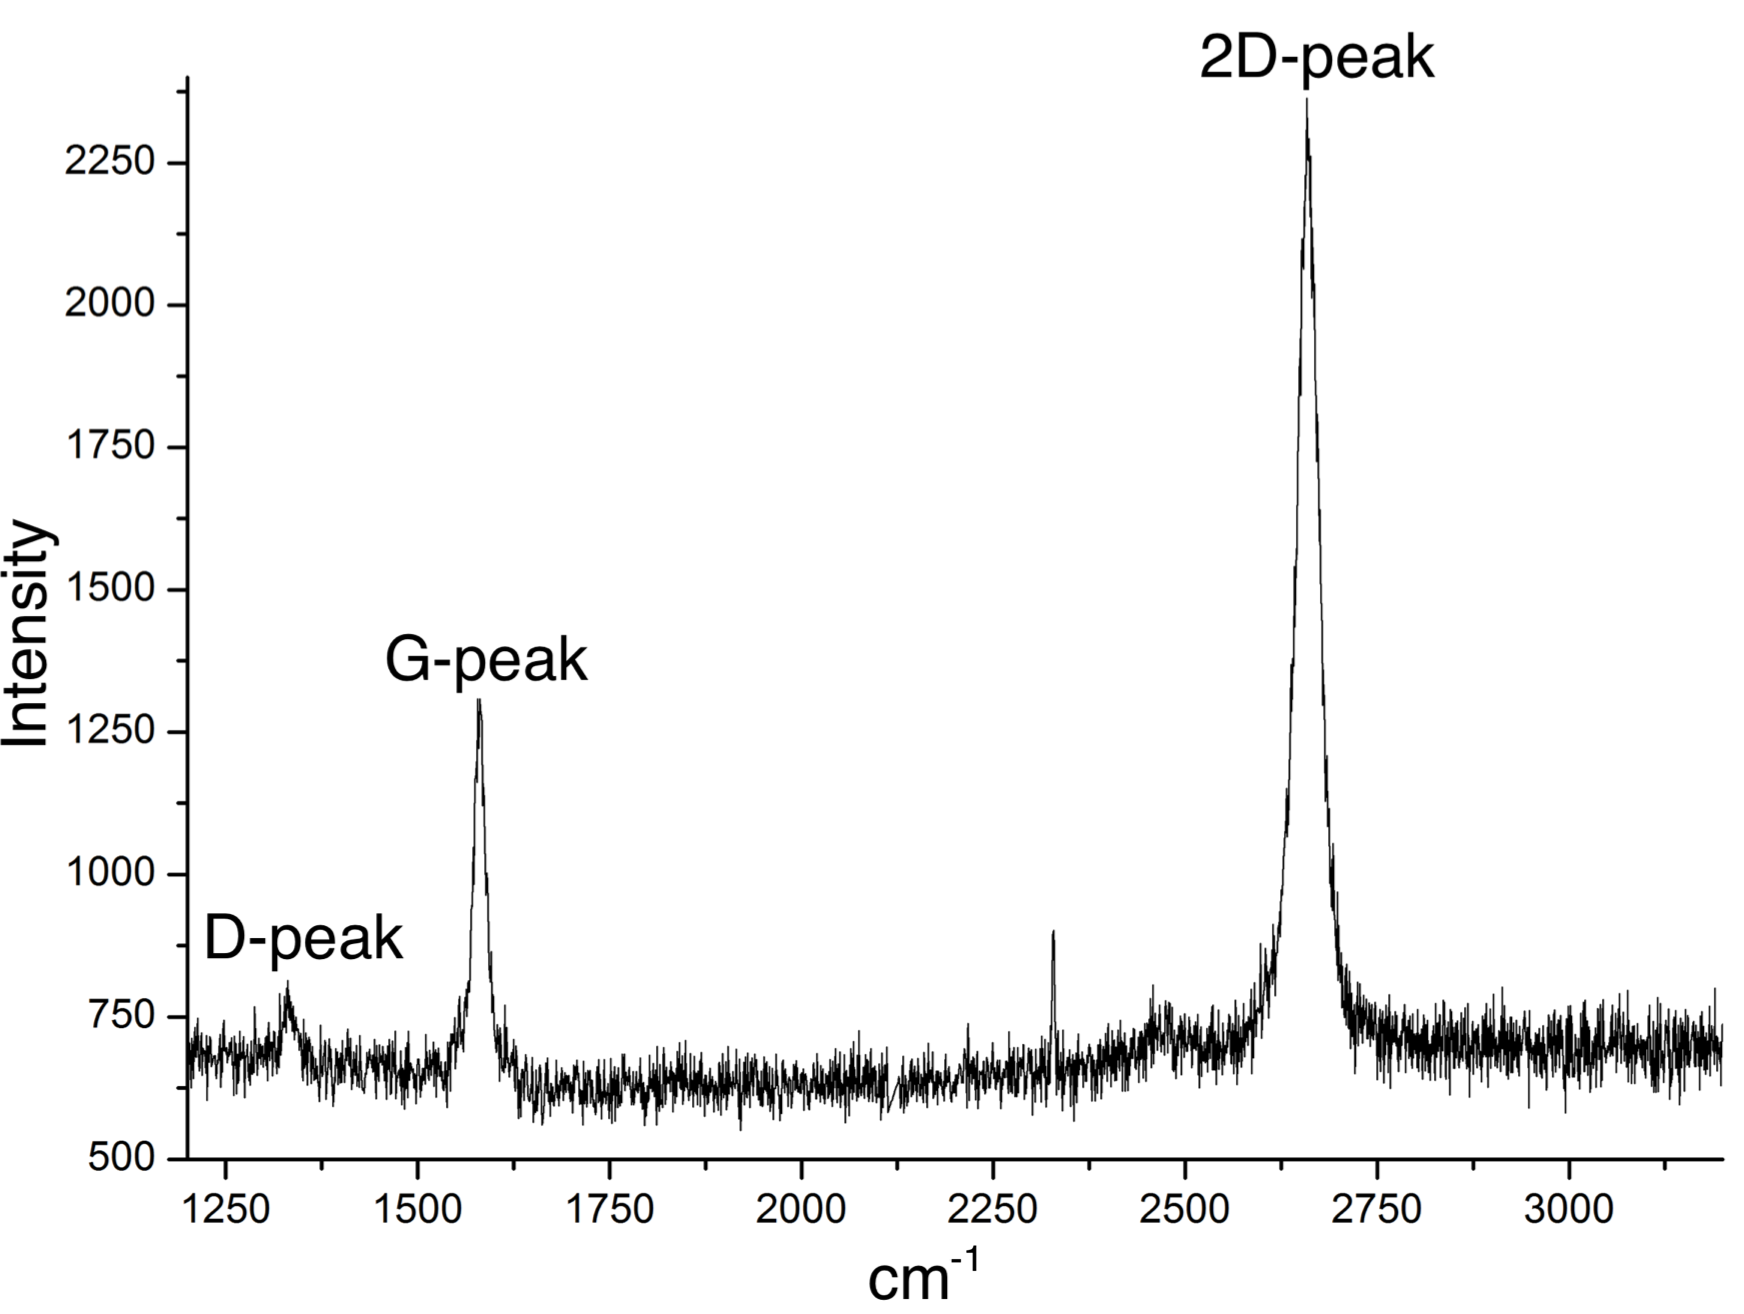
\includegraphics[width=0.7\textwidth]{./images/graphene-raman.png}
  \caption{The Raman spectrum of graphene showing the $D$, $G$ and $2D$ modes (adapted from \mcite, \note{add new image here}).}
  \label{fig:dispersion}
\end{figure}

Corresponding to a graph of the electronic band structure of graphene it is also possible to define a phononic band structure as shown in figure~\ref{fig:phonons}. Due to its two atom unit cell the phonon dispersion relation has three optical (O) and three acoustic branches (A). The phonon modes perpendicular to the plane are called out-of-plane (o) in contrast to in-plane modes (i). For further classification vibrations perpendicular and parallel to the axis of the two atoms in the unit cell are called transverse (T) and longitudinal (T).

\begin{figure}[!h]
  \centering
  \begin{subfigure}{0.7\textwidth}
    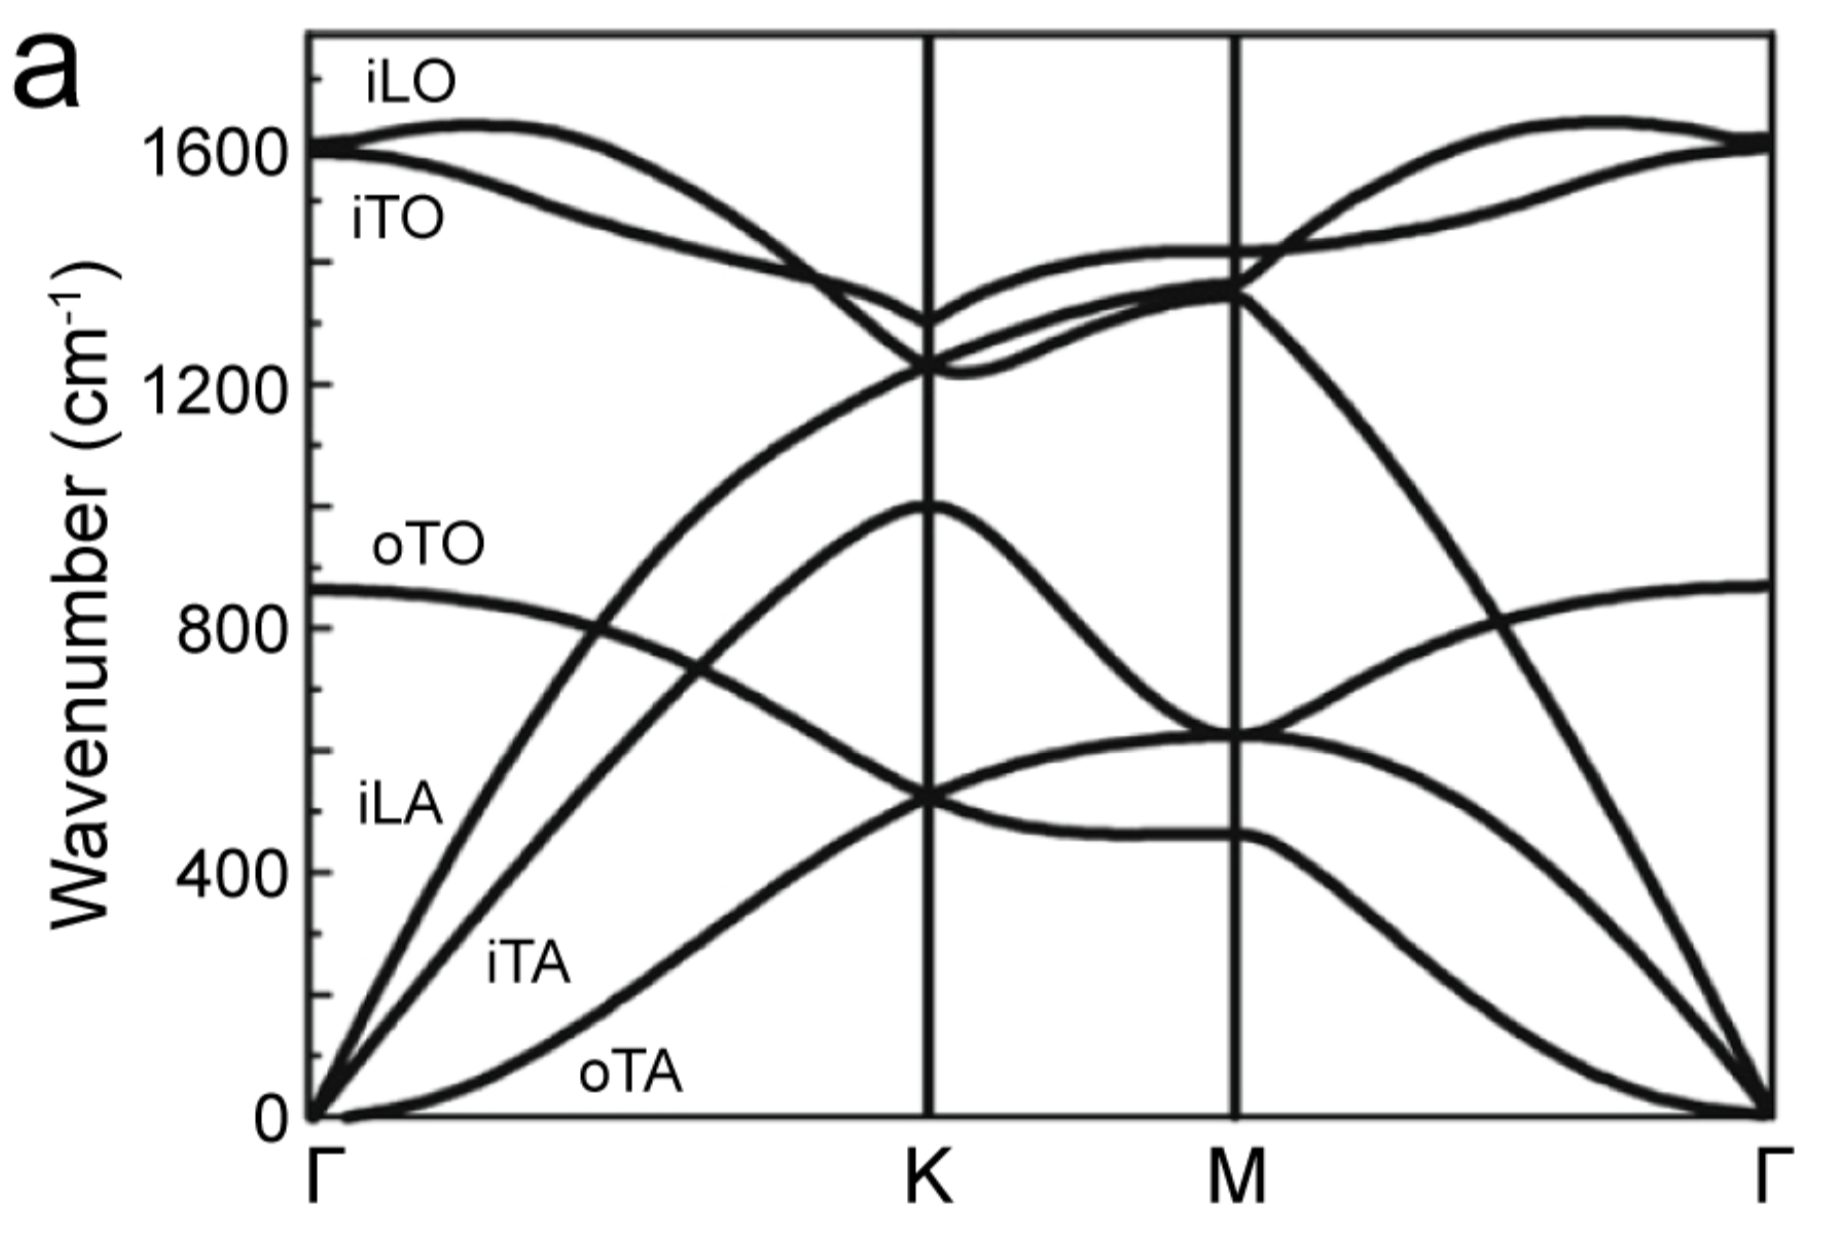
\includegraphics[width=\textwidth]{./images/phonon-modes.png}
  \end{subfigure}
  ~
  \begin{subfigure}{0.25\textwidth}
    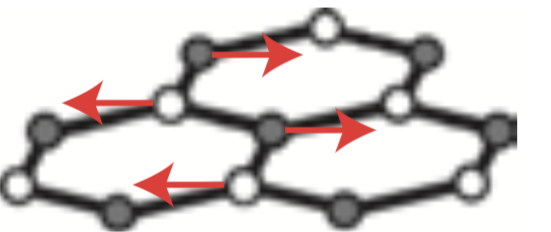
\includegraphics[width=\textwidth]{./images/g-mode-phonon.png}
    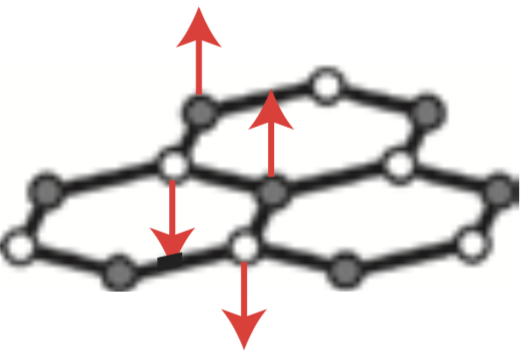
\includegraphics[width=\textwidth]{./images/g-mode-phonon-2.png}
    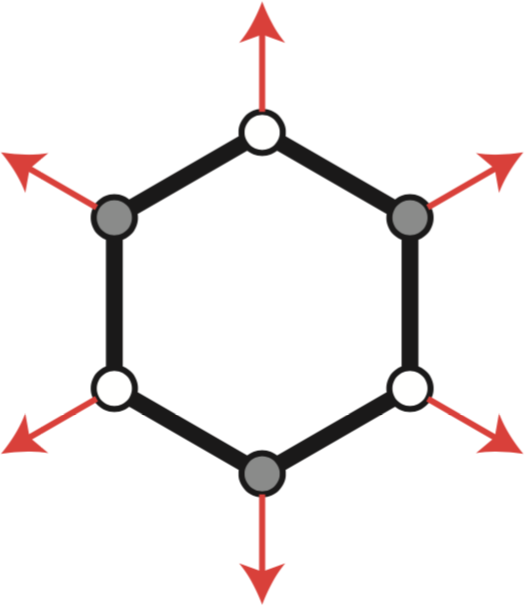
\includegraphics[width=\textwidth]{./images/2d-mode-phonon.png}
  \end{subfigure}
  \caption{\textbf{(a)}Calculated phonon dispersion relation of graphene along the $\Gamma$-$K$-$M$-$\Gamma$-direction with six phonon branches (Figure adapted from Malard et al. 2009\mcite). \textbf{(b)} $\Gamma$ point displacement pattern for graphene, causing the $G$-peak in graphene's Raman spectrum. ($E_{2g}^{(1)}$ and $E_{2g}^{(2)}$) \textbf{(c)} Displacement at $K$ causing the $2D$-peak in graphene's Raman spectrum ($A_2$).}
  \label{fig:phonons}
\end{figure}

\newpage

Interesting points in this band structure are the intersection of iLO and iTO bands at the $\Gamma$ point for the $G$ peak and at the $K$ points for the $2D$ peak.

\begin{figure}[!h]
  \centering
  \begin{subfigure}{0.2\textwidth}
    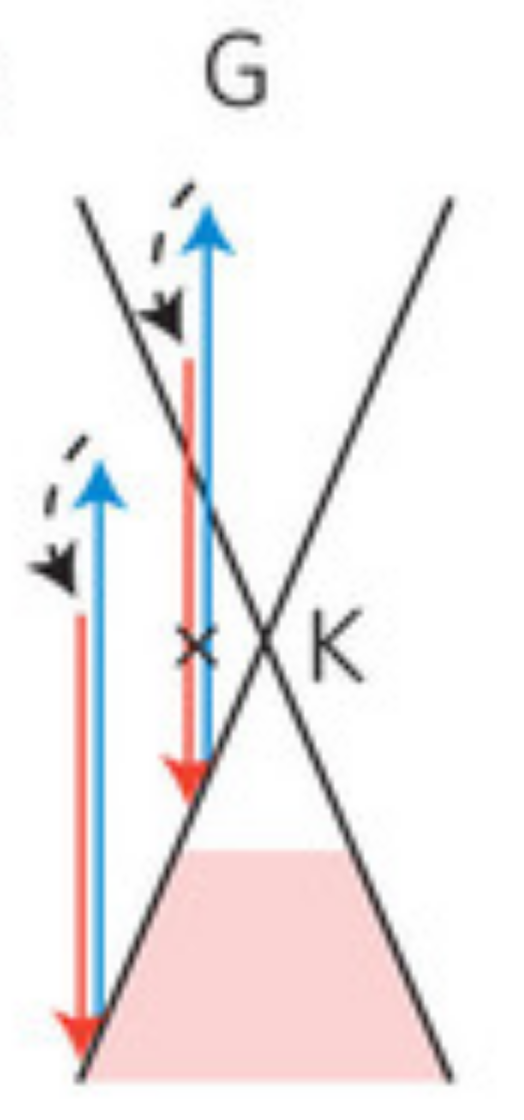
\includegraphics[width=\textwidth]{./images/g-mode.png}
  \end{subfigure}
  ~
  \begin{subfigure}{0.45\textwidth}
    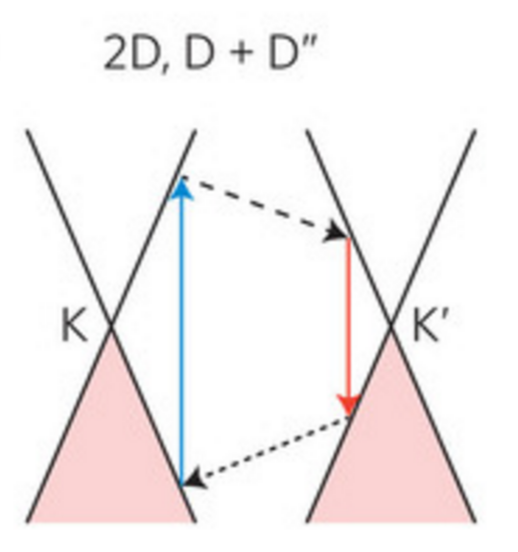
\includegraphics[width=\textwidth]{./images/2d-mode.png}
  \end{subfigure}
  \caption{Raman scattering processes for the $G$ and $2D$ peak of graphene. The band structure close to the K points is approximated as cones. \textbf{(a)} A photon is absorbed (blue arrow), scatters with a phonon (dashed arrow) and then is emitted with a lower frequency (red arrow), causing the $G$ peak in graphenes Raman spectrum. \textbf{(b)} A photon is absorbed (blue arrow), then scatters with two phonons (dashed arrows) and is emitted at a lower frequency (red arrow). This is the most prominent feature of graphene's Raman spectrum. \note{redraw this without forbidden transitions}}
  \label{fig:raman-modes}
\end{figure}

The most prominent featre in the Raman spectrum of graphene is its $2D$ which appears ats the $D$ peak overtone at ca \SI{2700}{cm^{-1}}. Two iTO phonons at the $K$ point with opposite wavevectors are involved in the scattering process to satisfy the momentum conservation as shown in figure~\ref{fig:raman-modes}. This mode does not require a defect for activation and therefore is always visible in graphene's spectrum.

At \SI{1582}{cm^{-1}} in the spectrum the $G$-peak is visible which is created by the iLO and iTO phonon bands \mcite. This corresponds to vibrations of the two sublatices consisting of the different base atoms against each other. In group theory it belongs to the tow-dimensional $E_{2g}$ representation \mcite.
